\documentclass[tikz,border=6pt]{standalone}
\usepackage{amsmath}
\usetikzlibrary{arrows.meta,positioning}
\usepackage[dvipsnames]{xcolor}

\begin{document}
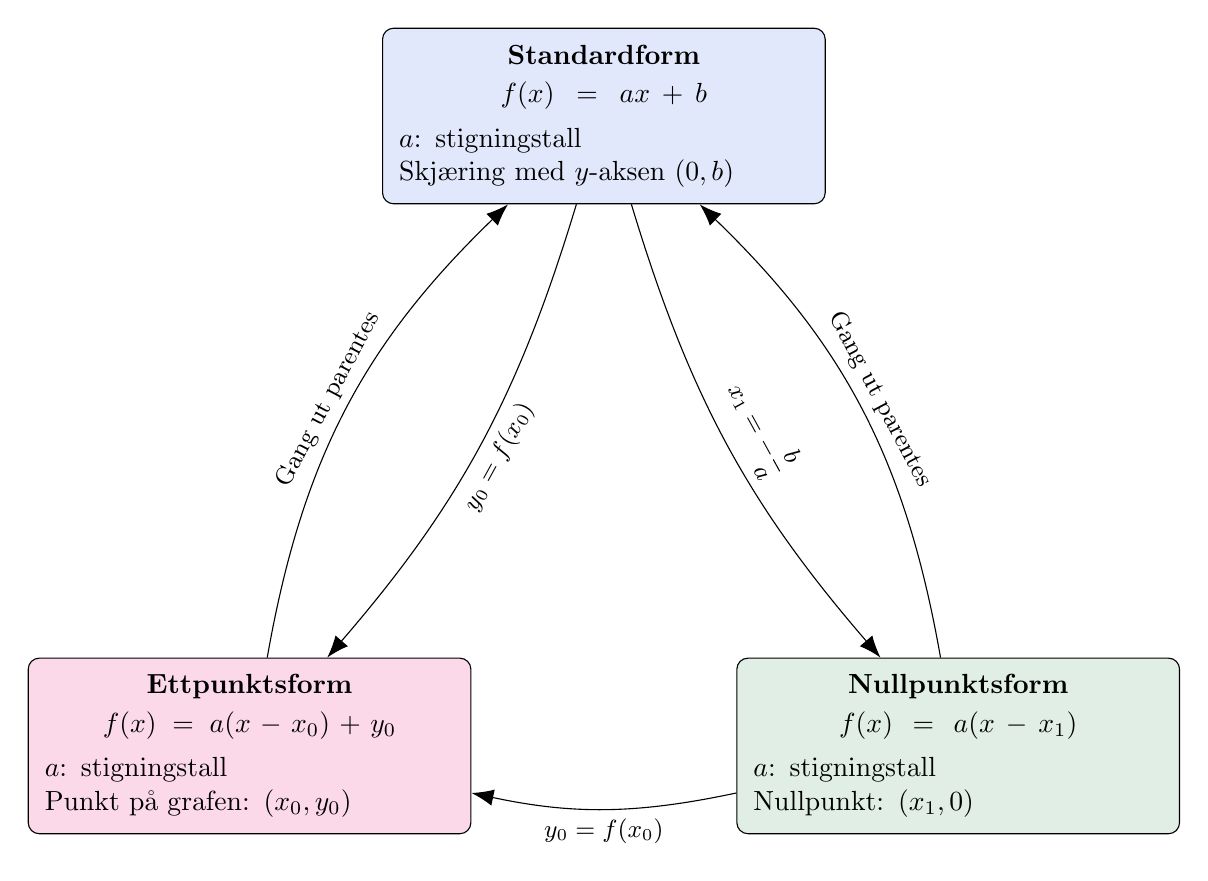
\begin{tikzpicture}[
  >={Latex[length=2.8mm]},
  box/.style   = {
    draw, rounded corners,
    align=center,
    inner sep=6pt,
    minimum width=\boxw,
    text width=\boxw,   % prevent width from growing
    fill=black!3
  },
  label/.style = {font=\small, align=center}
]

% ---- constants ----
\def\L{9}            % triangle side length
\def\H{8}          % height ~ (sqrt3/2)*L
\def\boxw{52mm}       % fixed width for every box

% ---- nodes (equilateral triangle) ----
\node[box, fill=RoyalBlue!15] (std) at (0,\H) {
  \textbf{Standardform}\\[2pt]
  $f(x)=ax + b$\\[4pt]
  % selectively left-align these two lines:
  \makebox[\boxw][l]{\normalsize $a$: stigningstall}\\
  \makebox[\boxw][l]{\normalsize Skjæring med $y$-aksen $(0, b)$}\\
};

\node[box, fill=RubineRed!15] (ext) at (-\L/2,0) {
  \textbf{Ettpunktsform}\\[2pt]
  $f(x)=a(x-x_0)+y_0$\\[4pt]
  \makebox[\boxw][l]{\normalsize $a$: stigningstall}\\
  \makebox[\boxw][l]{\normalsize Punkt på grafen: $(x_0, y_0)$}\\
};

\node[box, fill=SeaGreen!15] (nul) at (\L/2,0) {
  \textbf{Nullpunktsform}\\[2pt]
  $f(x)=a(x-x_1)$\\[4pt]
  \makebox[\boxw][l]{\normalsize $a$: stigningstall}\\
  \makebox[\boxw][l]{\normalsize Nullpunkt: $(x_1, 0)$}\\
};

% ---- arrows (circular-style bends) ----
\draw[->] (std) to[bend left=12]
  node[label,midway,sloped,below] {$y_0=f(x_0)$}
  (ext);

% \draw[->] (ext) to[bend left=12]
%   node[label,midway,sloped,above] {$y_0 = f(x_0)$}
%   (nul);

\draw[->] (nul) to[bend left=12]
  node[label,midway,sloped,below] {$y_0=f(x_0)$}
  (ext);

\draw[->] (nul) to[bend right=18]
  node[label,midway,sloped,above] {Gang ut parentes}
  (std);

\draw[->] (ext) to[bend left=18]
  node[label,midway,sloped,above] {Gang ut parentes}
  (std);

\draw[->] (std) to[bend right=12]
  node[label,midway,sloped,above] {$x_1 = -\dfrac{b}{a}$}
  (nul);

\end{tikzpicture}
\end{document}